\documentclass[a4paper]{article}

\usepackage{graphicx}

\title{Risolutore di puzzle – Parte 1}
\author{Alberto Andeliero}
\date{21 gennaio 2015}
\begin{document}
\maketitle
\centerline{Programmazione concorrente e distribuita}
\centerline{Progetto A.A. 2014/2015}
\section{Scelte progettuali}
PuzzleSolver come da specifica è stato concepito per modellare una realtà di puzzle rettangolari e di risolverne l'ordine delle tessere. Inoltre questo programma è stato pensato e progettato per essere estendibile con altre tipologie di puzzle rettangolari che trattino altri oggetti anzichè Stringhe al proprio interno. Quindi oltre alla classe PuzzleSolver che conterrà il main dell'applicazione, è stata modellata la classe Puzzle che è responsabile delle operazioni quali lettura da file di input, scrittura in file di output, e fondamentale il metodo sort che riordina i tasselli del puzzle secondo quanto richiesto dalla specifica tecnica.

\section{Organizzazione delle classi}
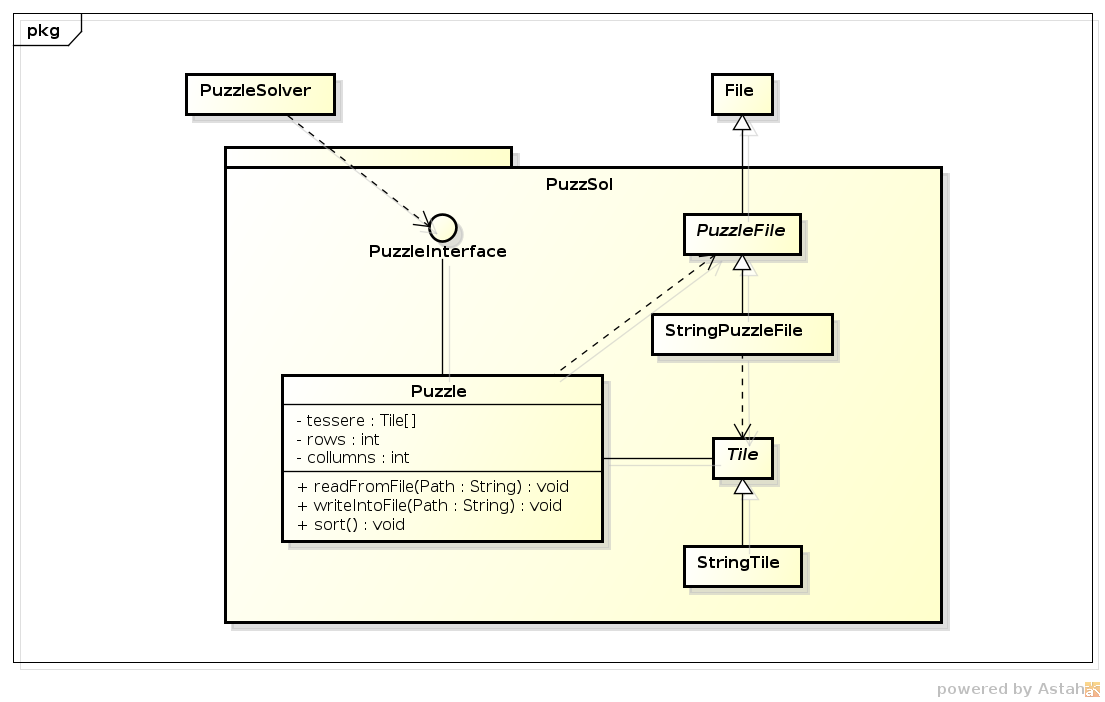
\includegraphics[width=\textwidth]{classdiagram.png}
Macroscopicamente possiamo vedere 3 gerarchie di classi, la gerarchia del Puzzle, la gerarchia delle tessere, ed infine la gerarchia dei PuzzleFile. La gerarchia della classe puzzle è composta da PuzzleInterface e da Puzzle, si è deciso di fornire un'interfaccia generica per avere una futura estensibilità con altre tipologie di puzzle ed inoltre per la creazione di un'istanza concreta di Puzzle è stato utilizzato un pattern di tipo Factory. La gerarchia delle tessere è composto semplicemente da una super classe astratta Tile che implementa già le operazioni di base e di confronto fra tessere e StringTile concretizza il fatto che la tessere è costituita da un'oggetto stringa. Infine abbiamo la gerarchia dei FilePuzzle dove PuzzleFile estende la classe File e StringPuzzleFile concretizza PuzzleFile implementando i metodi astratti di input e output utilizzati dalla classe Puzzle. Tutte le gerarchie sono state incapsulate nel package puzzsol tranne PuzzleSolver per ovvi motivi.

\section{Algoritmo di risoluzione}
Nella classe Puzzle possiamo trovare tutta la logica di ordinamento fondamentale alla risoluzione del puzzle. Avendo il riferimento a tutte le tessere lette in input da file, e il numero di colonne e di righe precedentemente calcolato,
\begin{enumerate}
\item In primis cerca il primo tassello in 0-posizione verificando che per ogni tassello presente vi sia uno con nord e ovest vuoti;
\item Successivamente il flusso procede a cercare il tassello più a est di quello precedentemente trovato, fino a completare l'intera riga;
\item Completata la riga si procede a cercare la tessera più a sud del capo riga;
\item Si ripete dal punto 2 il flusso fino a che tutte le righe non sono complete.
\end{enumerate}   
Nella classe interna TileScout sono state incapsulate tutti i metodi per la ricerca utili per l'algoritmo di risoluzione.

\section{Corettezza del programma}

\end{document}